\chapter{Characterisation of the electronic setup}

\textit{By the time the \gls{rf} signal has reached the acoustic transducer,
it has been synthesized from a reference signal, amplified, and matched to
the impedance of the \gls{aod} transducer. We are going to inspect the
\gls{rf} signal characteristics at each transmission and find that each stage
unintentionally carries out frequency dependent amplitude characteristics
which, as we will see in the next chapter, are responsible for the complex
intensity distribution observed with the photodiode.}

\section{Digital signal synthesizer}

We already covered the fundamental functionality of the \gls{dds} in
\cref{ch:digital_signal_synthesis} and its integration in our experimental
setup in \cref{subsec:setup_signal_source}, yet we are missing physical
measurements of the frequency and the amplitude characteristics.

Physical analysis of the \gls{dds} output \gls{rf} signal is in fact no simple
endeavour as usual operation time scales are of many magnitudes greater than
the signal periodicity. The strategy we used to resolve this circumstance is
depcited in \Cref{fig:signal_window}.
\begin{figure}[ht]
  \centering
  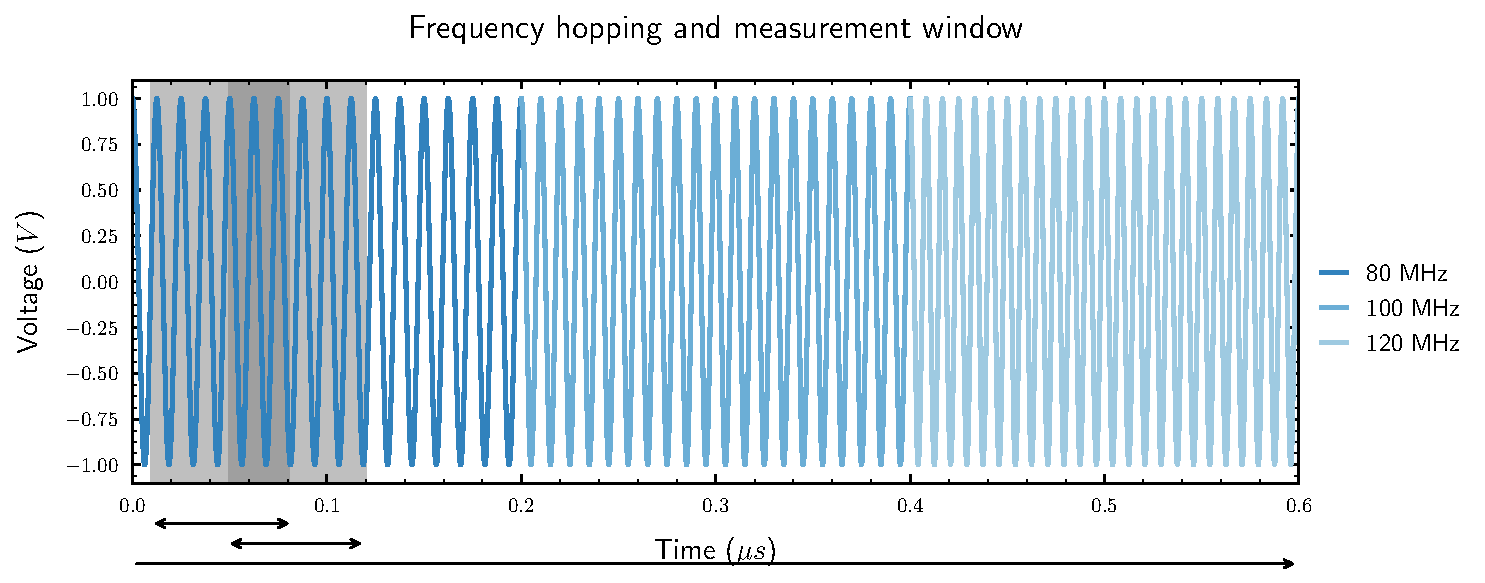
\includegraphics[width=\textwidth]{\figuredir{signal/window.pdf}}
  \captionsetup{width=.9\textwidth}
  \caption{Idealized \gls{dds} signal output with constant frequency
    increments. The measured window only captures a subset (gray) of the complete
    modulation (shades of blue).}\label{fig:signal_window}
\end{figure}
The strategy consists of capturing multiple, small time windows of the signal
(gray) which delayed would cover the complete signal trace (blue).
\begin{figure}[ht]
  \centering
  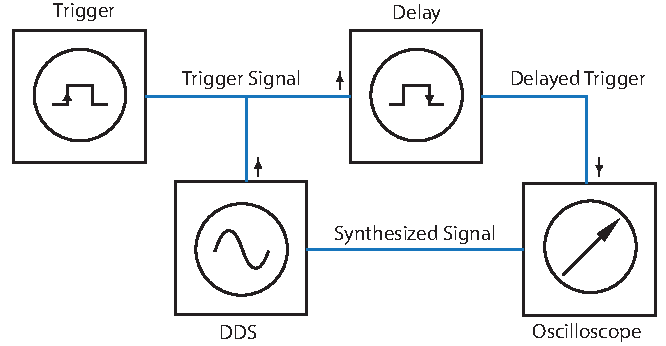
\includegraphics[width=.8\textwidth]{\figuredir{signal/setup-dds.pdf}}
  \captionsetup{width=.8\textwidth}
  \caption{Measurement setup of the synthesiyer signal. By inserting a pulse
    generator in between the trigger source and the oscilloscope we can delay
    the capture window of the oscilloscope by the pulse width.
  }\label{fig:signal_window_setup}
\end{figure}
The experimental setup used to reailize this concept is schematically drawn in
\Cref{fig:signal_window_setup}. In between the oscilloscope and the trigger
source we inserted a pulse generator. The pulse generator width equals the
delay time of the oscilloscope as the oscilloscope is configured to capture
on the falling edge signal of the pulse generator. Further the oscilloscope's
impedance was configured to \SI{50}{\ohm}. High impedance measurements at
such frequencies causes very different behaviour as the electromagnetic wave
is reflected subject to the actual frequency inside the coaxial cable. In 
\Cref{tab:signal_parameters_dds} we can find an overview of the experimental
parameters used.
\begin{table}[ht]
  \centering
  \begin{tabular}{|c|c|c|c|c|c|}
    \hline
    Frequency Range $f$ &
    Sweep Duration $T_s$ &
    Window Duration $T_w$ &
    Number Windows $N_w$ \\
    \hline
    \SIrange{80}{120}{\mega\hertz} &
    \SI{30}{\milli\second} &
    \SI{50}{\micro\second} &
    300 \\
    \hline
  \end{tabular}
  \captionsetup{width=.8\textwidth}
  \caption{Experimental parameters used to inspect the output \gls{rf} signal
    of the \gls{dds}.
  }\label{tab:signal_parameters_dds}
\end{table}
The specified frequency range is motivated to cover the greatest possible
spatial dimensions permitted by the dimensions of the optics. Sweep and
window duration where selected as a compromise between the oscilloscope being
able to resolve the signal fine enough to perform \gls{fft} and the sweep
duration being comparable to later experiments. Time delay was incremented
in $N_w$ steps until $T_s=T_w$, thus we will capture $N_w$ overlapping windows.

\subsubsection{Frequency spectrum}

For an ideal linear frequency sweep we would expect a continous increase of
the frequency with respect to time, yet we know that \gls{dds} makes use of
digital signal processing methods which suggests a discrete frequency
spectrum. To help us expose the characteristics of the digital frequency
sweep we will utilize a spectrogram. A spectrogram visualizes how the
frequency spectrum varies in time. One way to obtain a spectrogram is to
partition the data into overlapping time chunks while performing \gls{fft}
which allows us to combine time and frequency domain specific
characteristics. In our case we choose the relative spectral power to be
encoded through color.
\begin{figure}[ht]
  \centering
  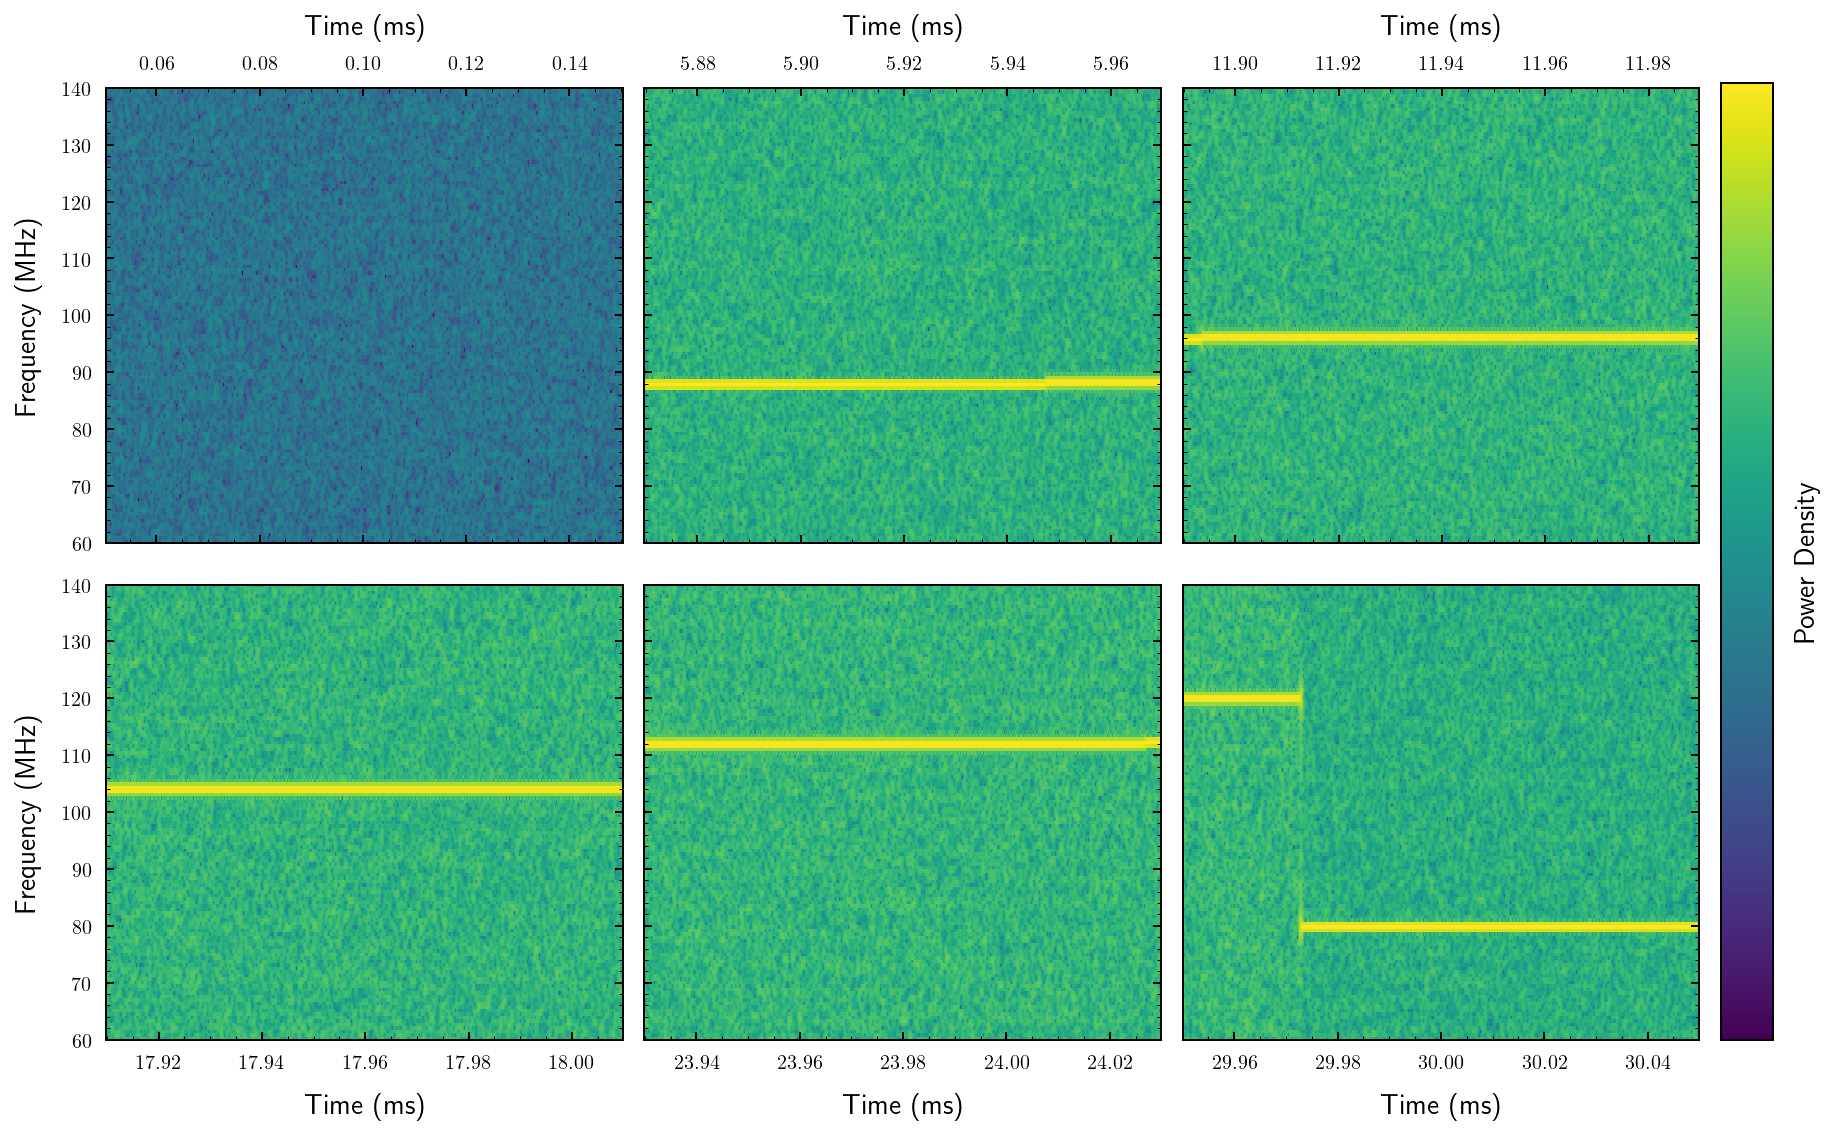
\includegraphics[width=\textwidth]{\figuredir{signal/synthesis/spectrogram.png}}
  \captionsetup{width=.8\textwidth}
  \caption{Spectrogram of delayed time windows of the \gls{dds} output signal
    configured to perform a linear frequency sweep. For an ideal linear sweep
    we would expect a linear timeline of the frequency, instead we observe a
    discrete set of frequencies.
  }\label{fig:signal_synthesis_spectrogram}
\end{figure}
\Cref{fig:signal_synthesis_spectrogram} depicts four spectrograms, each taken
at a different time window of the frequency sweep passthrough. The first
spectrogram captures the start of the frequency sweep as can be read from
the time scale. The first time window does not disclose any signal. This
phenomena will be observed frequently. For unknown reasons the output signal
of the \gls{dds} is absent for multiple microseconds after the \gls{dds}
receives the external trigger signal. The exact duration of the trigger hole
varies but does not affect the internal state of the \gls{dds} as the first
measured frequency matches the theoretically expected frequency according to
the ramp. If we take a look at the following spectrogram windows we can see
how the \gls{dds} outputs a constant frequency over a short time period,
therefore the frequency range consists of discrete frequencies. We can
actually even observe such a frequency increment in the second, third and
fifth spectrogram. Finally in the last spectrogram the frequency drops back
to the initial value --- a side effect of the \gls{dds} sweep mode which
supports an external trigger signal.

\subsubsection{Amplitude frequency response}

In the Fourier space we can locate the dominant frequency at the maximum of
the power spectrum. That in mind we can reduce the previous obtained time
window measurements to pairs of dominant frequencies and maximum amplitude.
Under the assumption that the maximum voltage per measurement is approximately
the mean peak-to-peak amplitude of the signal --- which during the
oscilloscope suggested during measurements --- we can find the amplitude
frequency response spectrum with manageable effort.
\Cref{fig:signal_synthesis_response} visualizes the described routine for the
\gls{dds} assigned to the \gls{h} and \gls{v} \gls{aod} with frequency control
by digital ramp and manual increments.
\begin{figure}[ht]
  \centering
  \includegraphics[width=.9\textwidth]{\figuredir{signal/synthesis/response.pdf}}
  \captionsetup{width=.9\textwidth}
  \caption{Amplitude frequency response of the \gls{dds} signal sources for
    the \gls{h} and \gls{v} \gls{aod}. The frequency increments
    are performed through the integrated digital ramp and manually.
  }\label{fig:signal_synthesis_response}
\end{figure}
The peak-to-peak amplitude of the synthesizser signal is constant with small
noise contribution. On a closer view we can see that the oscilloscopes voltage
resolution is at its limit, thus we only observe discrete voltage steps.
We therewith conclude from \Cref{fig:signal_synthesis_response} that the
amplitude response of the \gls{dds} is independent of the output frequency
and the method used to provide frequency increments. The inverse sinc response
we theorized in \cref{ch:digital_signal_synthesis} is not observable in the
measured frequency range as \SI{100}{\mega\hertz} are a fraction of the
Nyquist frequency \SI{1}{\giga\hertz} used for sampling inside the \gls{dds}.

\section{Power amplifier}

The piezoelectric attached to the acousto-optic crystal inside the \gls{aod}
elements has to emit acoustic waves strong enough to propagate through the
crystal of the \gls{aod}. The power demands specified by the \gls{aod} are
not met by the \gls{dds}, therefore we have to employ a power amplifier
between the \gls{dds} and \gls{aod}. Even though we previously concluded that
the \gls{dds} signal amplitude is independent of the output frequency, the
power amplifier can introduce new frequency dependent characteristics which
we dedicate ourselves to.

\subsubsection{Amplitude frequency response}\label{subsec:electronic_amplitude_frequency_response}

The measurement procedure described in the previous section is still valid
for the now amplified signal of projected \SI{33}{\decibel\meter}. At the
usual \SI{50}{\ohm} in between coaxial cables this corresponds to an
approximate voltage of \SI{10}{\volt}. In order to protect the oscilloscope
against potential damage caused by too much power, we inserted a chain of
attentuators (order given from coaxial cable to oscilloscope):
\begin{inparaenum}
  \item \SI{1}{\decibel}
  \item \SI{3}{\decibel}
  \item \SI{3}{\decibel}
  \item \SI{6}{\decibel}
  \item \SI{10}{\decibel}
  \item \SI{10}{\decibel}
\end{inparaenum}
The order was chosen in such a way to distribute heat dissipation uniformly
accross the attentuators. The total damping of this configuration yields
\SI{33}{\decibel} which should give us the same signal power from the
\gls{dds}. \Cref{fig:signal_amplification_response} presents us the damped
output signal subject to the signal frequency after amplification for the two
distinct (\gls{h}, \gls{v}) amplifiers and \gls{dds} signals.
\begin{figure}[ht]
  \centering
  \includegraphics[width=.9\textwidth]{\figuredir{signal/amplification/response.pdf}}
  \captionsetup{width=.9\textwidth}
  \caption{Amplitude frequency response of the \gls{dds} signal after power
    amplification. In comparison to the \gls{dds} we observe very small
    oscillations.
  }\label{fig:signal_amplification_response}
\end{figure}
In comparison to the \gls{dds} response the amplifier introduce small ripple
around about \SI{97}{\mega\hertz} and \SI{107}{\mega\hertz}. Further we note
a small constant offset between the \gls{h} and \gls{v} amplifier. We also
cannot identify significant differences between the type of frequency
increment used. Despite these effects are small in terms of voltage it is
difficult to relate them to the overall power response as only voltage but
not current was measured.

\subsubsection{Network analyzer transmission}

We previously discovered that the amplifier amends the frequency amplitude
response, nevertheless it is difficult to isolate the actual influence of
the amplifier and to preclude interaction effects caused by the already
unideal \gls{dds} signal. Therefore we conducted more detailed measurements
of the amplifiers power transmission with the network analyzer. The network
analyzer is a device that can measure reflection and transmission parameters
of electric components and does provide a cleaner input signal then used in
the previous measurement. As in the measurement with the oscilloscope we also
have to protect the network analyzer against the output power of the
amplifier. This time we used a single \SI{30}{\decibel} attentuator in between
the network analyzer input and the power amplifier output.
\begin{figure}[ht]
  \centering
  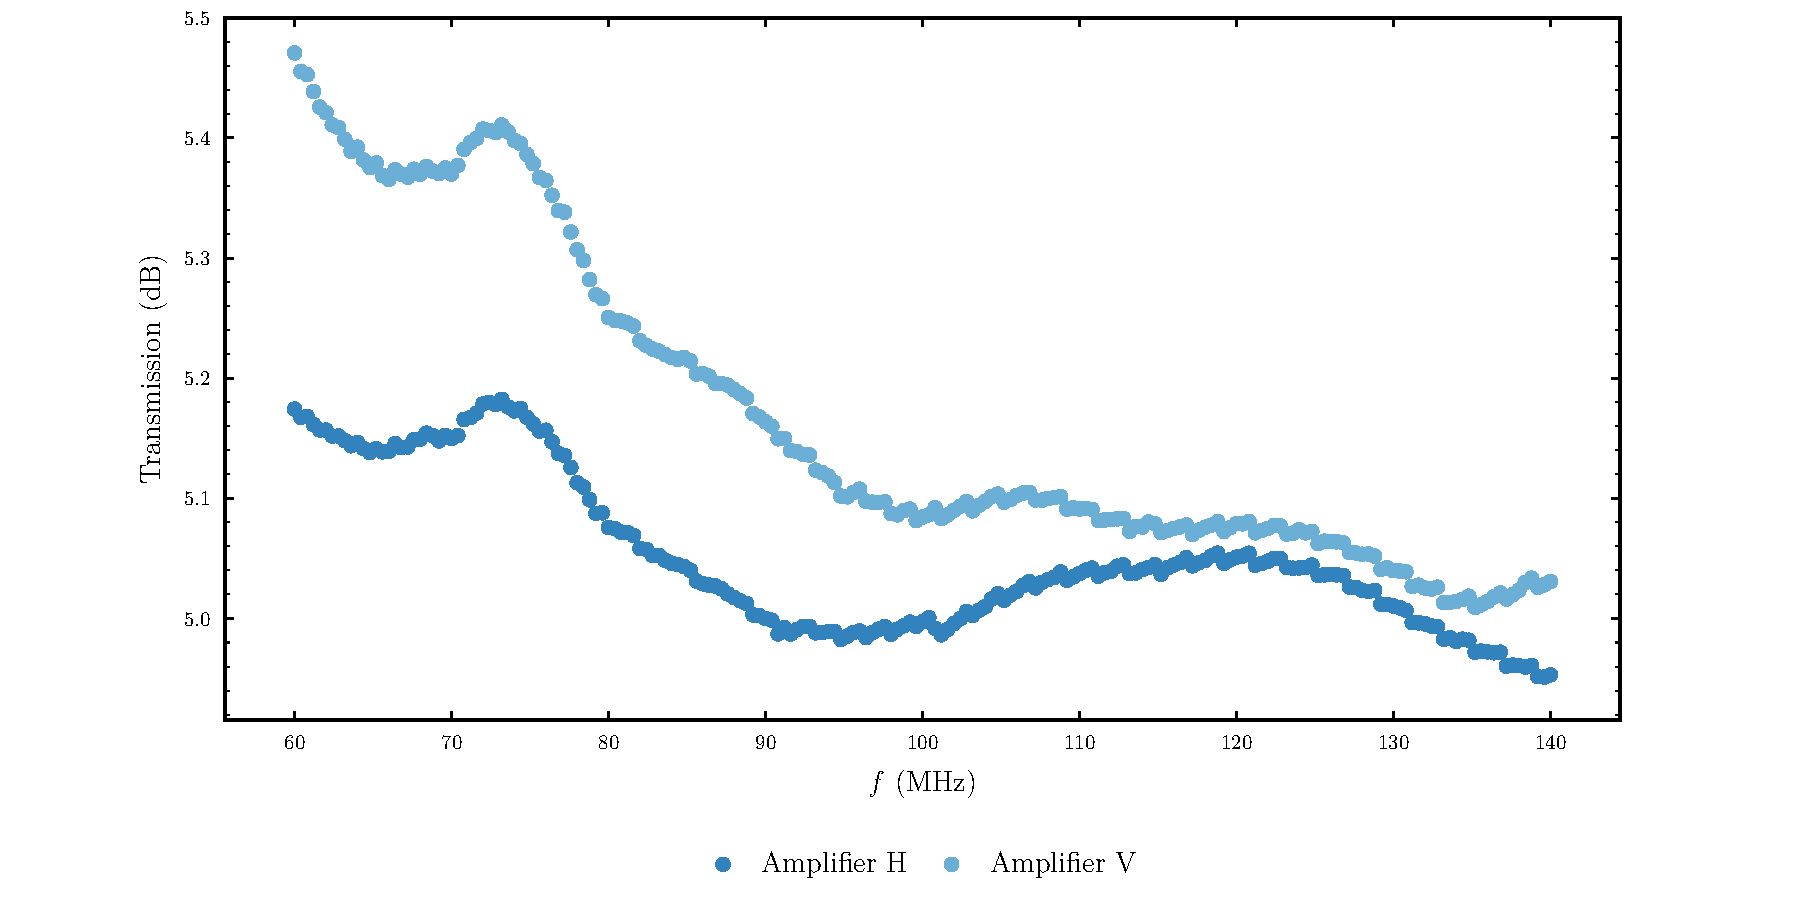
\includegraphics[width=.9\textwidth]{\figuredir{signal/amplification/transmission.pdf}}
  \captionsetup{width=.9\textwidth}
  \caption{Frequency transmission spectrum obtained via the network analyzer
    of the horziontal and vertical amplifiers.
  }\label{fig:signal_amplification_spectrum}
\end{figure}
In \Cref{fig:signal_amplification_spectrum} we see the frequency transmission
spectrum obtained through the network analyzer connected to the horizontal
and vertical amplifiers. We can confirm a fixed offset of the amplification
gain between both amplifiers. If we take a assume a power amplification
difference of $L=\SI{.2}{\decibel}$, i.e.\ between \SI{80}{\mega\hertz} and
\SI{115}{\mega\hertz} with the \gls{v} amplifier, according to
\begin{equation}
  P
  =
  P_0 10^{L/\SI{10}{\decibel}}
  \label{eq:power_gain_decibel}
\end{equation}
and $P_0=\SI{2}{\watt}$ we would have to expect a drop of up to
\SI{.05}{\watt} in power. Unfortunately we cannot say in how far this is
a relevant magnitude for the \gls{aod}.

\section{Acoustic transducer}

In the previous sections we explored the signal transfer at the synthesis
and amplification stage. The last stage that is accessable to us without
destruction of the \gls{aod} concerns the power reflection at the \gls{aod}
itself. From the reflection we may estimate power transmission
characteristics, hence for a large reflection we would expect a small
transmission and in that sense less beam intensity in the first deflection
order.

\subsection{Reflection spectrum}

The power reflection measurements were conducted with the network analyzer
we already introduced on the power amplifiers. In a first embodiment of the
experiment we directly supplied the \gls{aod} through a coaxial cable of the
network analyzer with power and measured the reflection. In a second
embodiment we used a direct-coupler to supply the respective amplifier with a
signal and measure the reflection through a direct-coupler.

\subsubsection{Direct connection}

\Cref{fig:signal_reflection_direct} visualizes the power reflection spectrum
of both \gls{aod} elements when directly connected to the network analyzer at
a maximum output power of \SI{10}{\decibel\meter}.
\begin{figure}[ht]
  \centering
  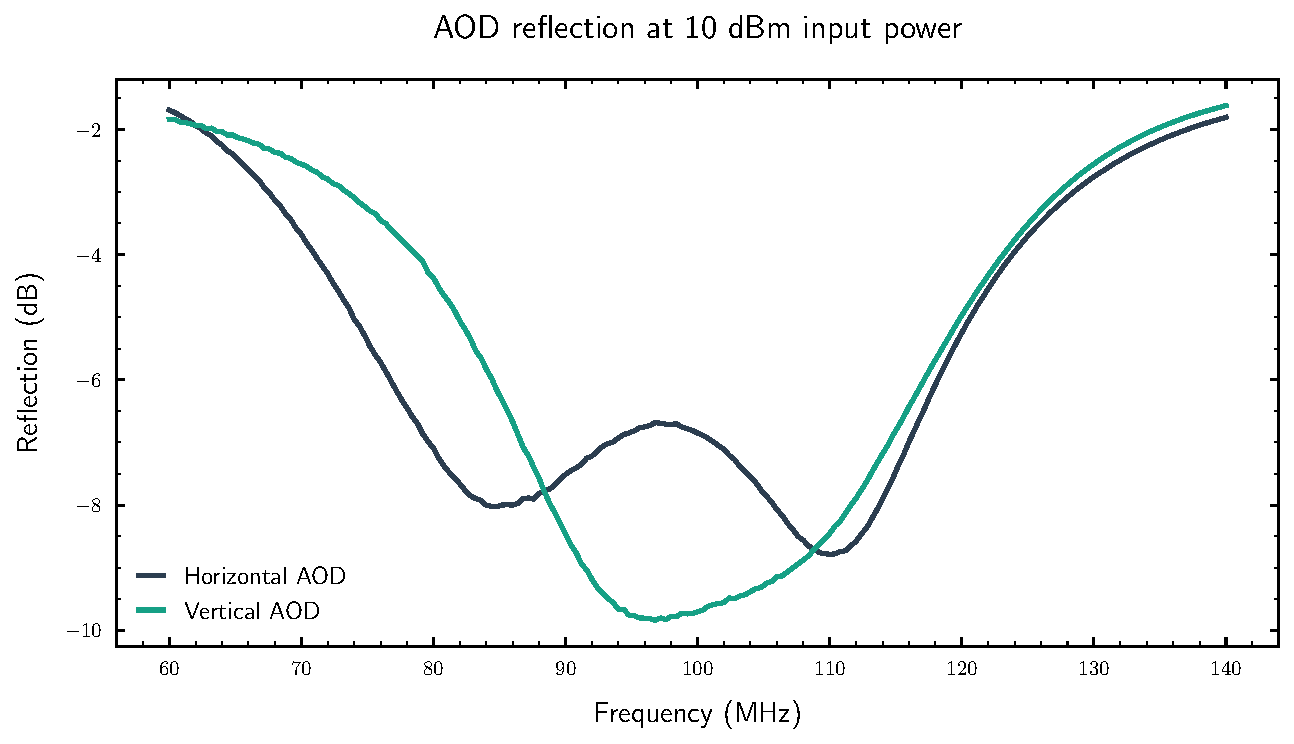
\includegraphics[width=.9\textwidth]{\figuredir{signal/reflection/direct.pdf}}
  \captionsetup{width=.8\textwidth}
  \caption{Signal reflection of the two different \gls{aod} when directly
    connected to the network analyzer.
  }\label{fig:signal_reflection_direct}
\end{figure}
The most interesting finding in \Cref{fig:signal_reflection_direct} is that
the power reflection shows very different behaviour in between the distinct
\gls{aod} elements. The \gls{aod} anticipated for the vertical deflection
is most transmissive at \SI{97}{\mega\hertz} with transmission falling of
on both sides while the \gls{aod} anticipated for the horizontal deflection
has two local transmission maxima and a rather bad transmision near the center
frequency.

\subsubsection{Amplified coupled connection}

In the second procedure we amplify the signal and couple the network analyzer
through a direct-coupler to measure the refleciton. This is done in order to
avoid harm to the network analyzer and because the network analyzer is not
able to provide \SI{2}{\watt} of output power as required by the \gls{aod}.
\begin{figure}[ht]
  \centering
  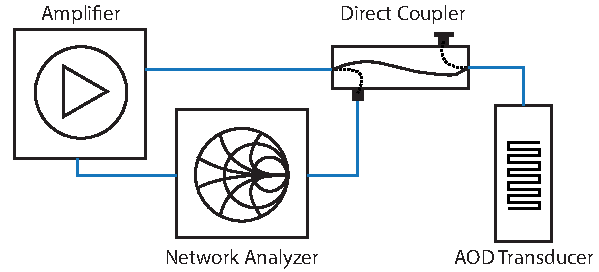
\includegraphics[width=.8\textwidth]{\figuredir{signal/setup-transducer.pdf}}
  \captionsetup{width=.8\textwidth}
  \caption{Experimental setup to measure the reflection at the acouso-optic
  transducer component. The network analyzer supplies an input signal to
  the amplifier. The output signal of the amplifier is connected through
  a direct-coupler with the acousto-optic element. The direct-coupler allows
  to safely measure input and output reflection.
  }\label{fig:signal_amplification_transducer_setup}
\end{figure}
The setup is depicted in \Cref{fig:signal_amplification_transducer_setup}.
The network analyzer on the left-hand side supplies an input signal to the
amplifier. The input signal changes linear in frequency. The output signal
of the amplifier is connected through a direct-coupler with the acousto-optic
element. The direct-coupler allows to measure input and output reflection.
\begin{figure}[ht]
  \centering
  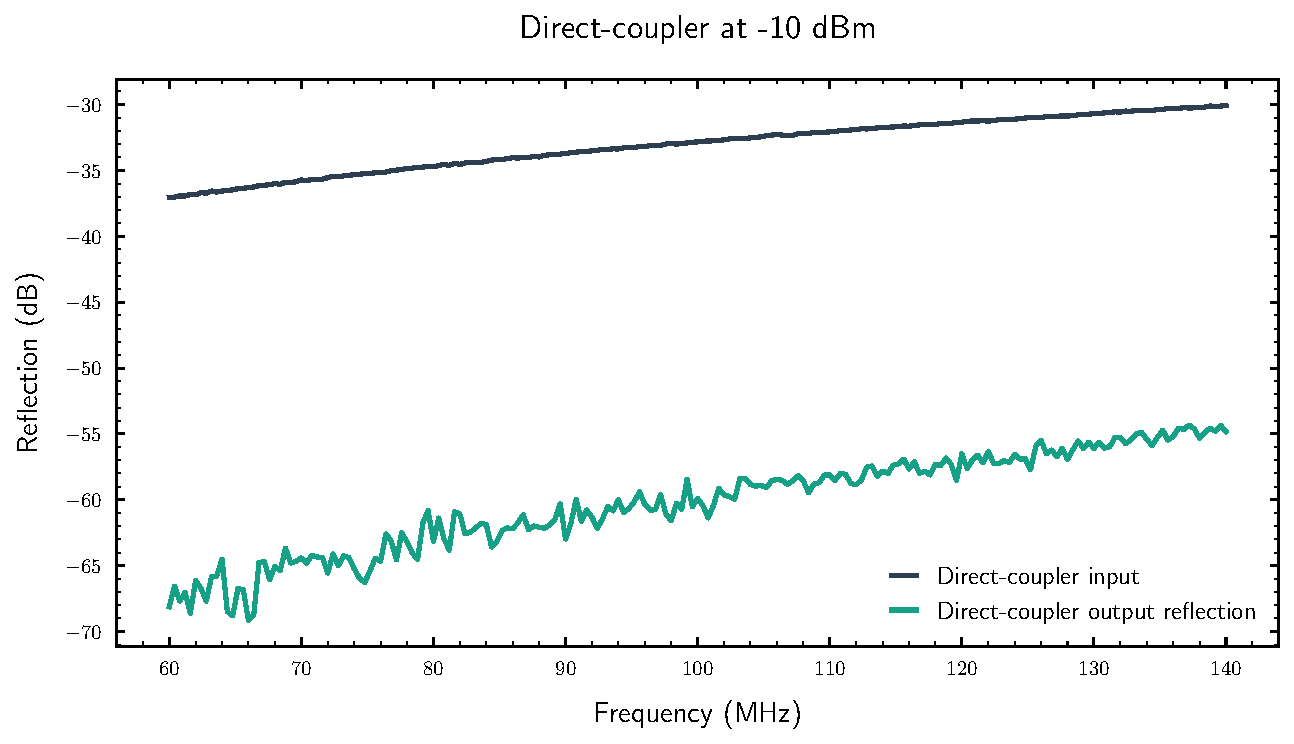
\includegraphics[width=\textwidth]{\figuredir{signal/reflection/coupler.pdf}}
  \captionsetup{width=.8\textwidth}
  \caption{Input power reflection when supplying the direct-coupler with
    \SI{-10}{\decibel\meter} input signal and reflection at the closed output
    of the direct-coupler while other ports are closed with \SI{50}{\ohm}.
  }\label{fig:signal_reflection_coupler}
\end{figure}
The direct-coupler is an apparatus comprising a coaxial input and output
port as well as a coaxial input reflection and output reflection port. It is
disignated to measure the reflection of a (possible) high power signal
without jeopardizing measurement equipement.
\begin{figure}[ht]
  \centering
  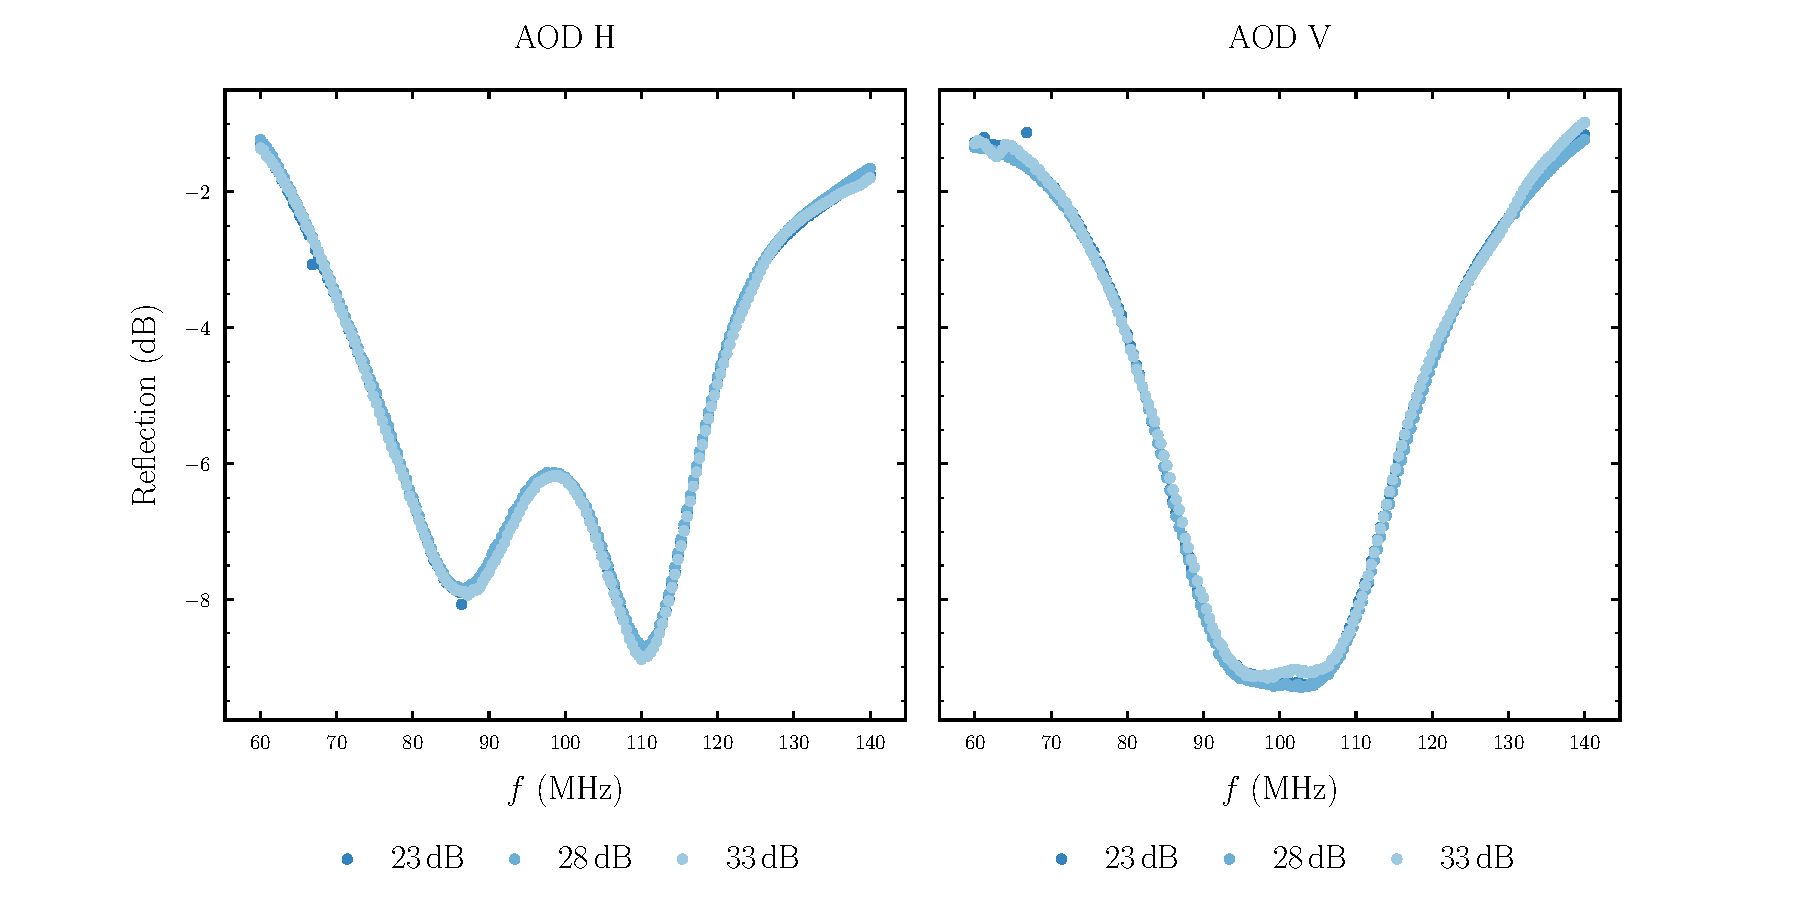
\includegraphics[width=\textwidth]{\figuredir{signal/reflection/coupled.pdf}}
  \captionsetup{width=.8\textwidth}
  \caption{Reflection at the direct-coupler output after amplification of the
  network analyzer input signal for different effective powers. We see that
the applied power does not effect the spectrum.
}\label{fig:signal_reflection_coupled}
\end{figure}
In \Cref{fig:signal_reflection_coupler} we see the reflection spectrum for
the case that we provide the network analyzer output signal to the input of
the direct-coupler and connect the reflection output of the direct-coupler
with the second network analyzer port while the remaining ports are under
\SI{50}{\ohm} closure.

We note that the reflection measured through the direct-coupler is lowered
by many orders of magnitude compared to the input signal but essentially of
the same shape. The noise in the reflection is very high because of the low
power supplied into the direct-coupler. We now use the direct-coupler to
measure the output reflection at the
\gls{aod} elements after the signal was amplified.

In \Cref{fig:signal_reflection_coupled} we see the effective reflection
spectrum for the distinct \gls{aod} elements. The effective reflection
spectrum is obtained when subtracting the input reflection from the output
reflection.

\subsubsection{Comparison}

In the previous part we saw that the reflection spectrum does not show any
power dependence, thus we should be able to compare the spectrum we obtained
directly with the amplified result.
\begin{figure}[ht]
  \centering
  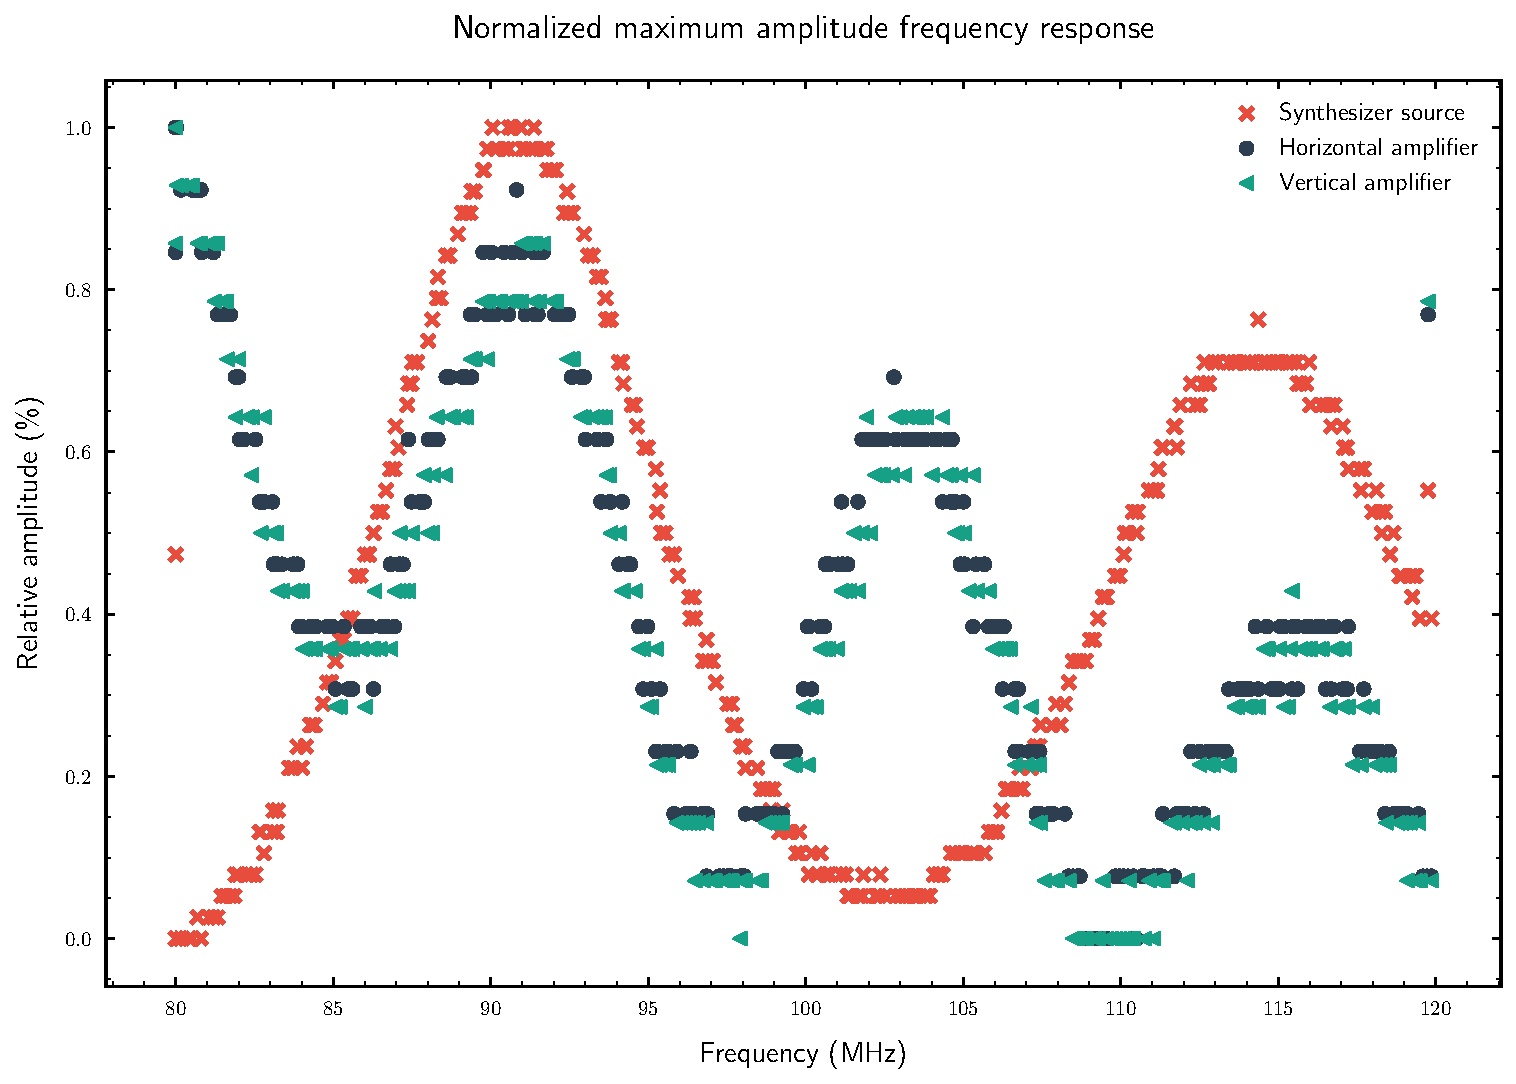
\includegraphics[width=\textwidth]{\figuredir{signal/reflection/comparison.pdf}}
  \captionsetup{width=.8\textwidth}
  \caption{Reflection from amplified input signal and direct signal as well as
    transmission from the amplifier spectrum.
  }\label{fig:signal_reflection_comparison}
\end{figure}
In \Cref{fig:signal_reflection_comparison} we can see how there is additional
reflection from the amplifier, nevertheless the global spectrum
characteristics stay in place.

\subsubsection{Summary}

Distinct \gls{aod} elements show different power transmission characteristics
independent of the applied power. Examination of the \gls{aod} elements in
details discloses different impedance matching circuits. Impedance matching
is used to reduce power reflection by providing a constant input resistance
of \SI{50}{\ohm} accross an ideally wide frequency range. Still the impedance
differs between the \gls{aod}s. We assume that the crystal properties
i.e.\ cut, purity are responsible for that, this is supported by the fact
that the impedance matching circuits differ between the \gls{aod} elements.
